\chapter{Measurement Results}

For this chapter different combinations of two links employing pure ALOHA, non-persistent CSMA and 1-persitent-CSMA-like MAC protocols were run on the same channel. In-depth analysis of different metrics and a consecutive protocol assessment are provided. 

\textbf{As a reminder:} If not specified otherwise all transmitters are backlogged. CSMA/CA throughout this thesis is not featuring the optional RTS/CTS exchange.

\section{Same Protocol Combinations}

Throughout this section both transmitters are executing identical flowgraphs. Generally, when both links use the same MAC protocol we expect to see comparable results for any over a sufficiently longer period of time, although small variations are also expected due to statistical and hardware-related effects and inaccuracies. 

\subsection{Pure ALOHA}

For two links with saturated ALOHA traffic we have zero throughput, since each and every package collides. 

\begin{figure}[tb]
	\label{fig:results-aloha-dbl}
	\begin{center}
		\centerline{
			\subfloat[throughput]{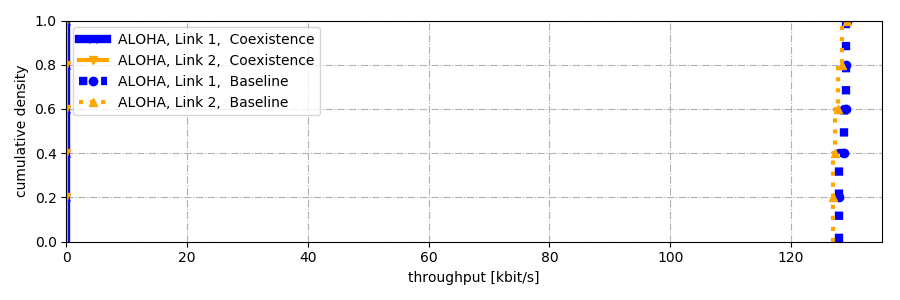
\includegraphics[width=0.6\textwidth]{pictures/results/same_combinations/aloha/throughput_cdf}}
			\subfloat[packet loss CDF]{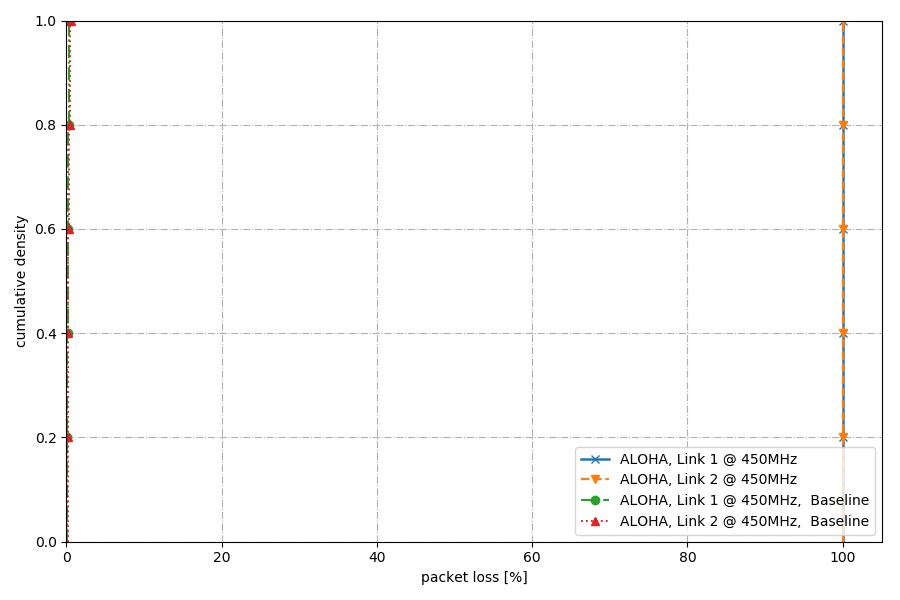
\includegraphics[width=0.6\textwidth]{pictures/results/same_combinations/aloha/packet_loss_cdf}}
		}
		\centerline{
			\subfloat[channel energy]{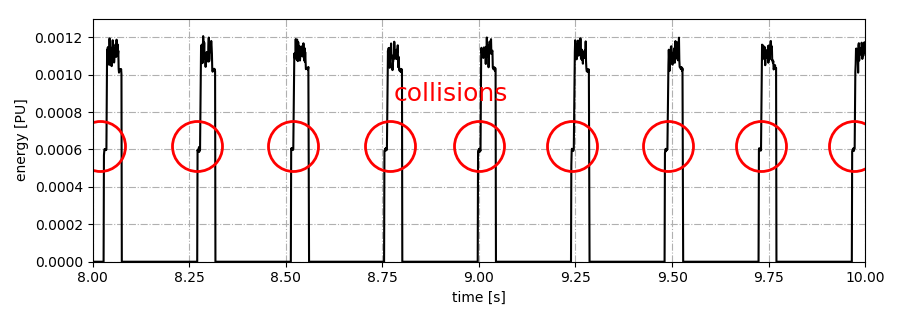
\includegraphics[width=0.6\textwidth]{pictures/results/same_combinations/aloha/smoothed_channel_energy_level_4_line_chart}}
			\subfloat[channel energy CDF]{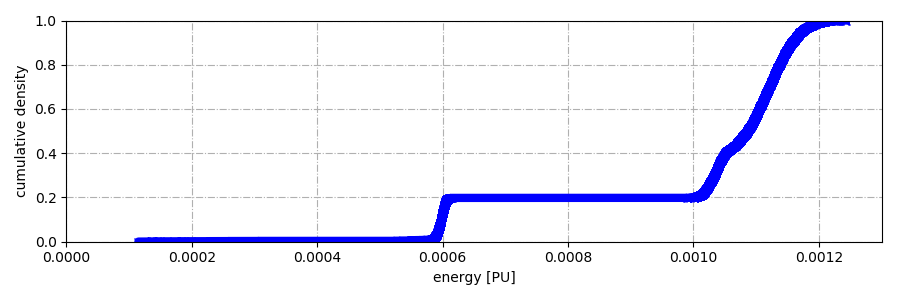
\includegraphics[width=0.6\textwidth]{pictures/results/same_combinations/aloha/smoothed_channel_energy_cdf}}
		}		
	\end{center}
	\caption{Measurement results for the CSMA/CA with large parameter set}
\end{figure} 

\clearpage



\subsection{CSMA/CA With High Parameter Set}

\begin{figure}[tb]
	\label{fig:results-csma-high-dbl}
	\begin{center}
		\centerline{
			\subfloat[throughput]{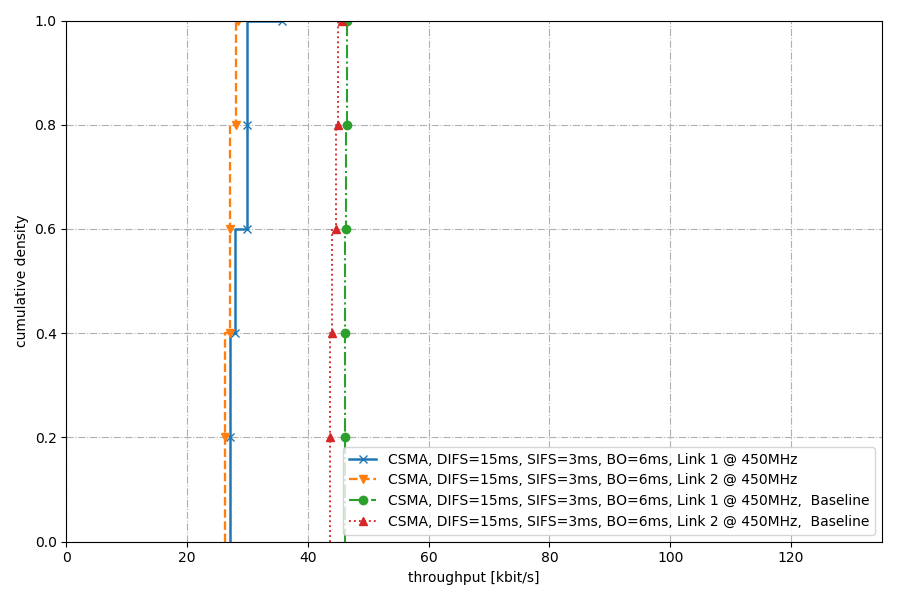
\includegraphics[width=0.6\textwidth]{pictures/results/same_combinations/csma_high_params/throughput_cdf}}
			\subfloat[frame delay]{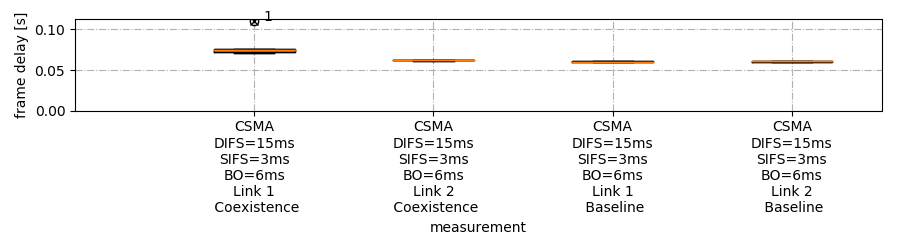
\includegraphics[width=0.6\textwidth]{pictures/results/same_combinations/csma_high_params/frame_delay_boxplot}}
		}
		\centerline{
			\subfloat[channel energy]{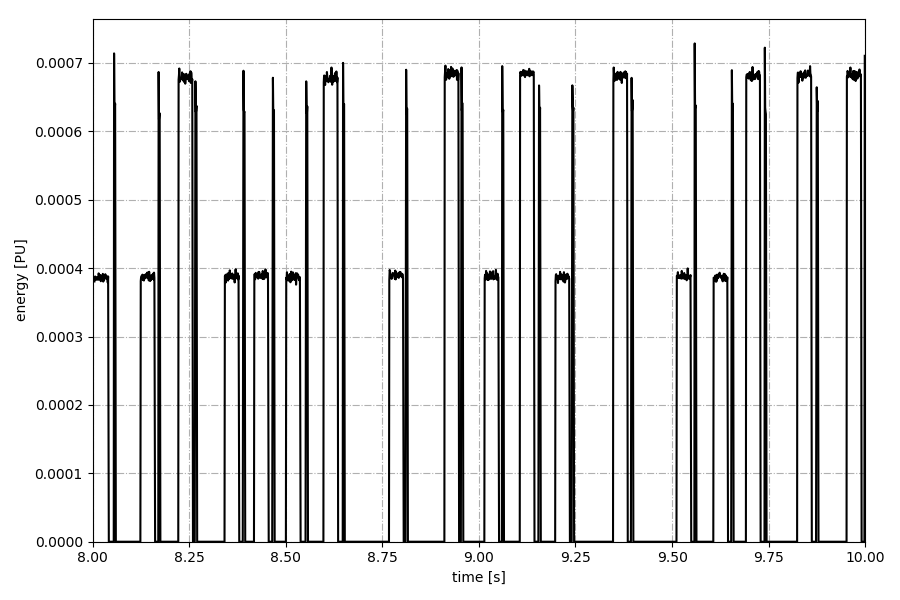
\includegraphics[width=0.6\textwidth]{pictures/results/same_combinations/csma_high_params/smoothed_channel_energy_level_4_line_chart}}
			\subfloat[channel energy CDF]{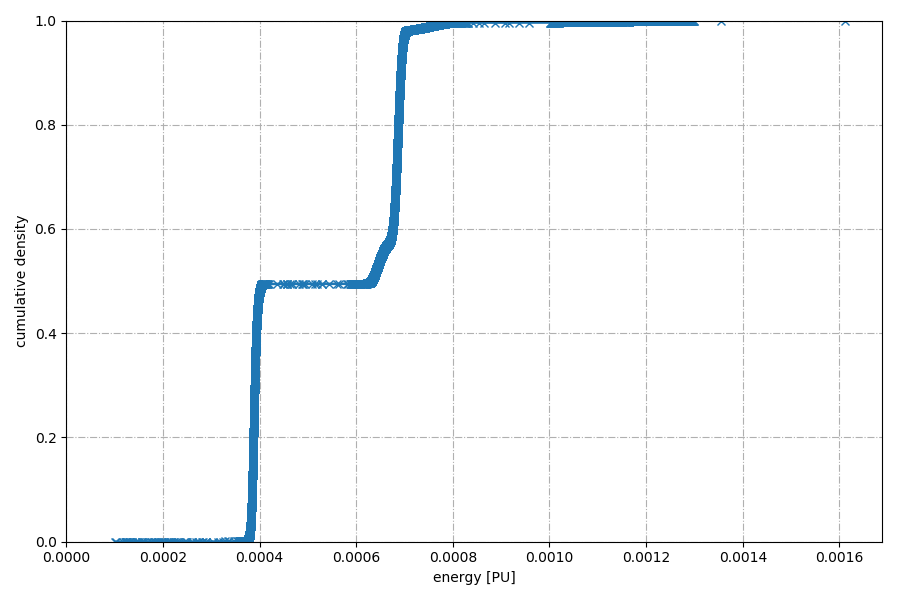
\includegraphics[width=0.6\textwidth]{pictures/results/same_combinations/csma_high_params/smoothed_channel_energy_cdf}}
		}
		\centerline{
			\subfloat[logical channel occupation]{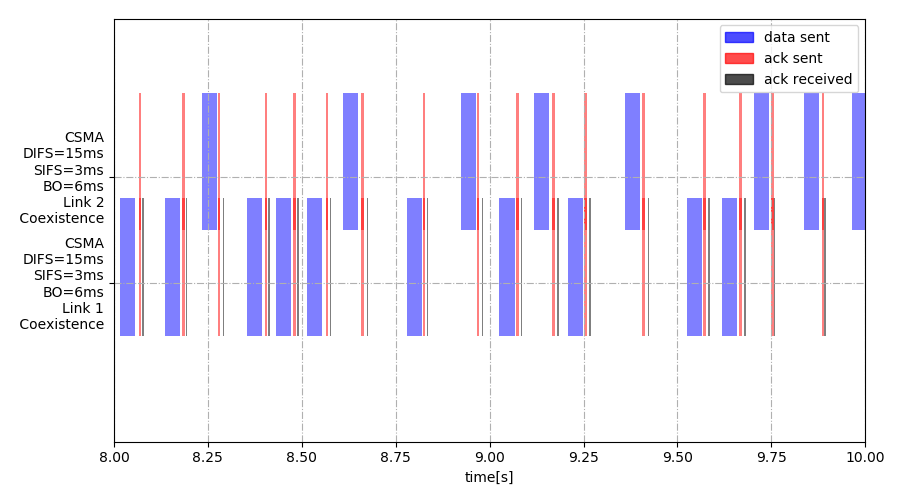
\includegraphics[width=0.6\textwidth]{pictures/results/same_combinations/csma_high_params/zoomed_channel_occupation_gantt_chart}}
			\subfloat[total backoff]{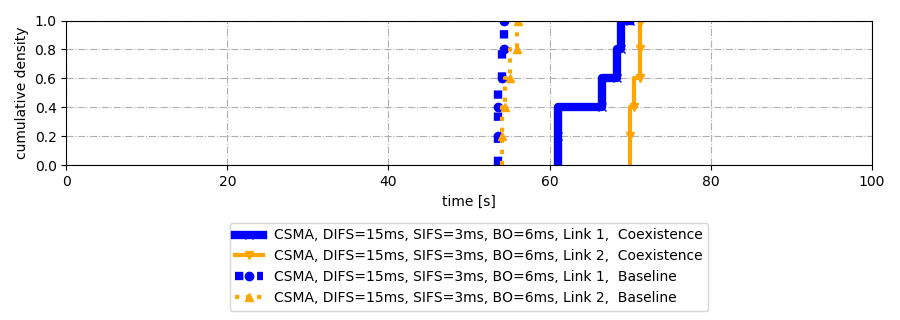
\includegraphics[width=0.6\textwidth]{pictures/results/same_combinations/csma_high_params/backoff_(joint)_sum_cdf}}
		}		
	\end{center}
	\caption{Measurement results for the CSMA/CA with high parameter set}
\end{figure}

\clearpage



\subsection{CSMA/CA With Low Parameter Set}

\begin{figure}[tb]
	\label{fig:results-csma-low-dbl}
	\begin{center}
		\centerline{
			\subfloat[throughput]{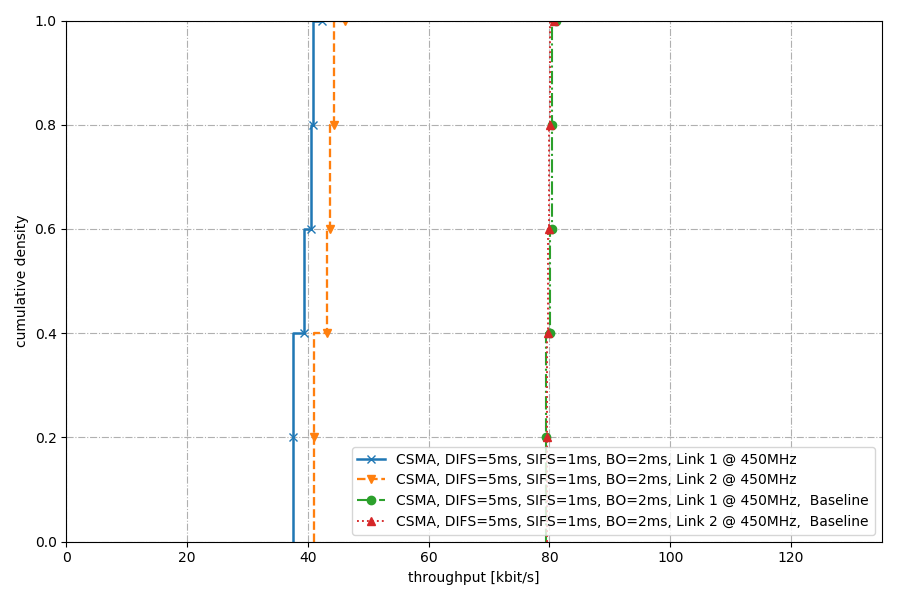
\includegraphics[width=0.6\textwidth]{pictures/results/same_combinations/csma_low_params/throughput_cdf}}
			\subfloat[frame delay]{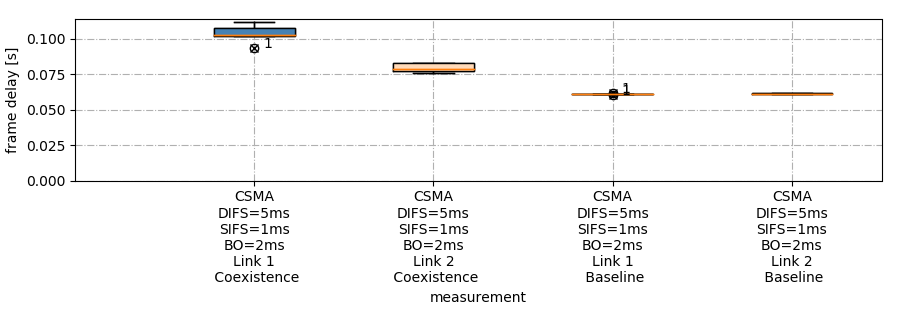
\includegraphics[width=0.6\textwidth]{pictures/results/same_combinations/csma_low_params/frame_delay_boxplot}}
		}
		\centerline{
			\subfloat[channel energy]{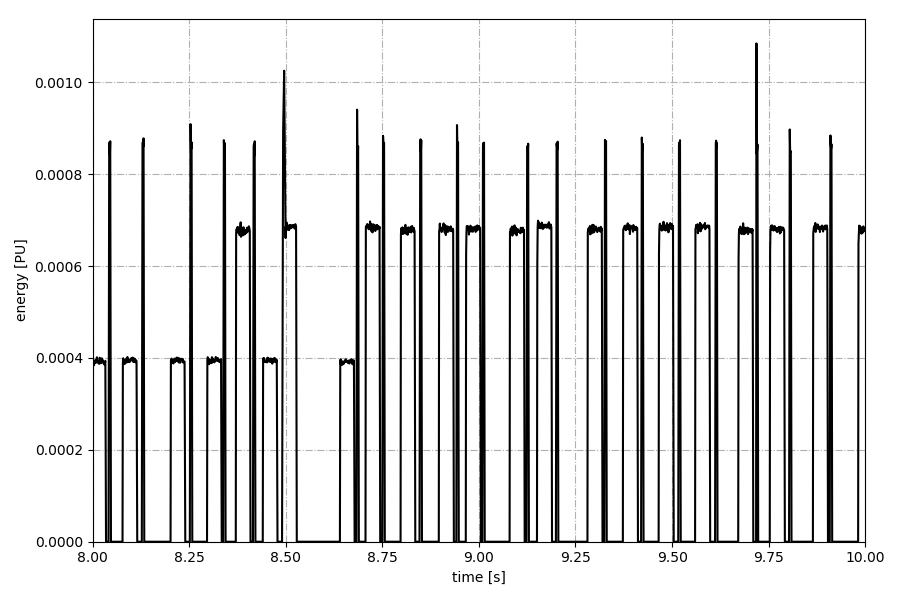
\includegraphics[width=0.6\textwidth]{pictures/results/same_combinations/csma_low_params/smoothed_channel_energy_level_4_line_chart}}
			\subfloat[channel energy CDF]{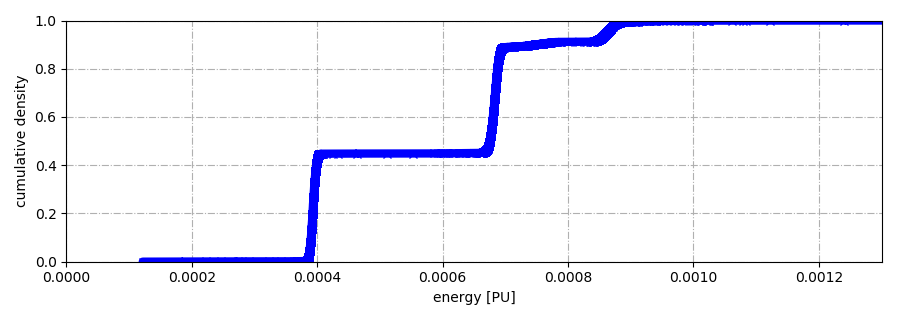
\includegraphics[width=0.6\textwidth]{pictures/results/same_combinations/csma_low_params/smoothed_channel_energy_cdf}}
		}
		\centerline{
			\subfloat[logical channel occupation]{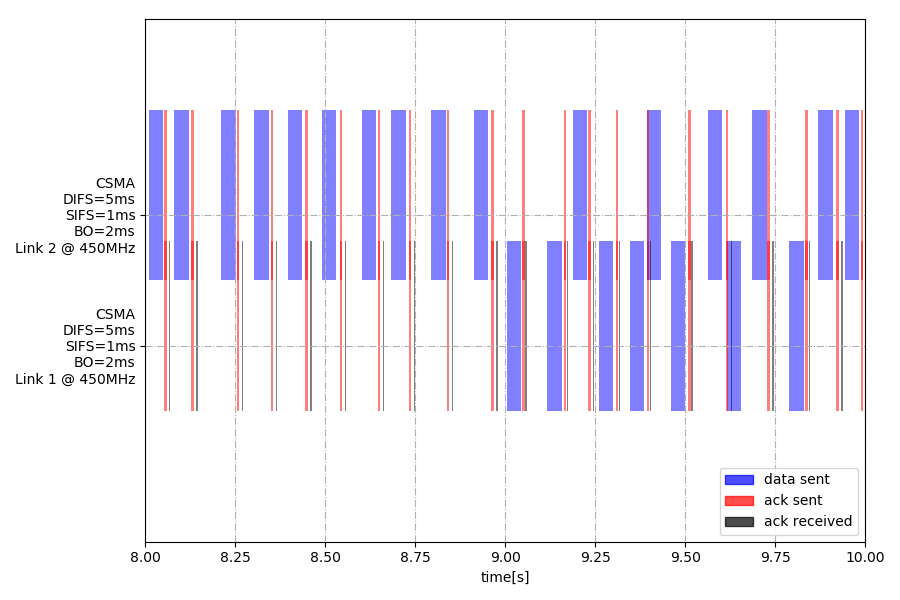
\includegraphics[width=0.6\textwidth]{pictures/results/same_combinations/csma_low_params/zoomed_channel_occupation_gantt_chart}}
			\subfloat[total backoff]{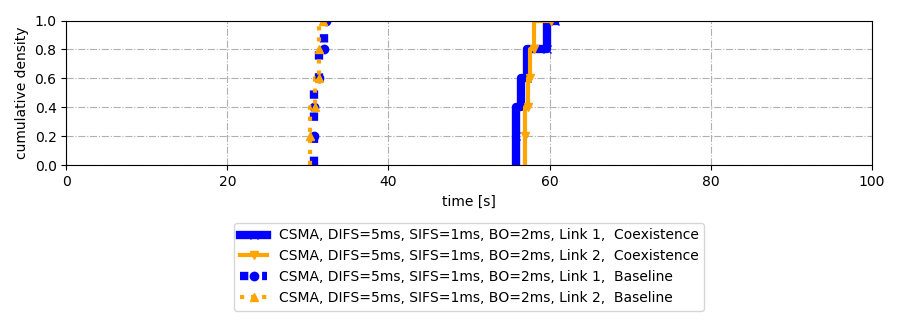
\includegraphics[width=0.6\textwidth]{pictures/results/same_combinations/csma_low_params/backoff_(joint)_sum_cdf}}
		}		
	\end{center}
	\caption{Measurement results for the CSMA/CA with low parameter set}
\end{figure}

\clearpage

\subsection{CSMA/CA With Medium Parameter Set}

\begin{figure}[tb]
	\label{fig:results-csma-med-dbl}
	\begin{center}
		\centerline{
			\subfloat[throughput]{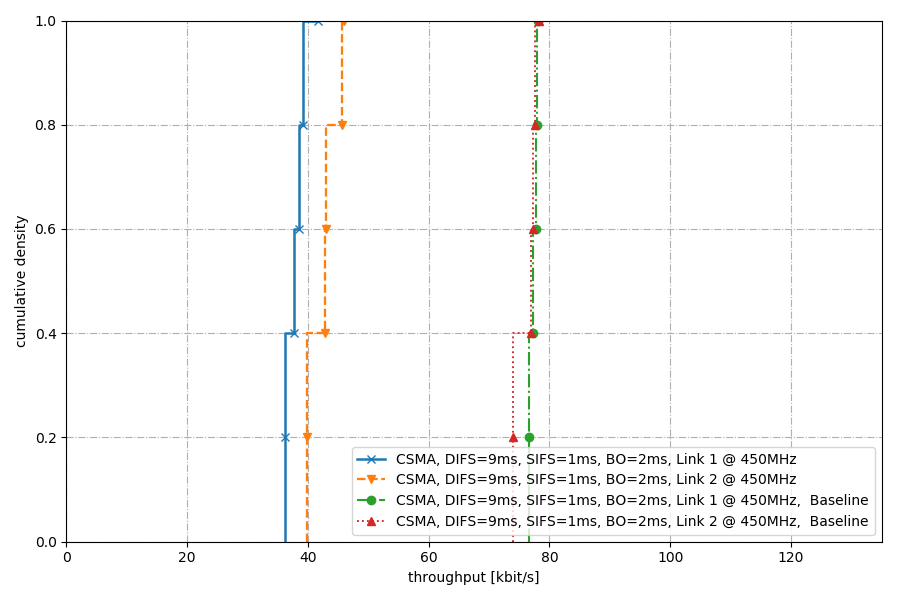
\includegraphics[width=0.6\textwidth]{pictures/results/same_combinations/csma_med_params/throughput_cdf}}
			\subfloat[frame delay]{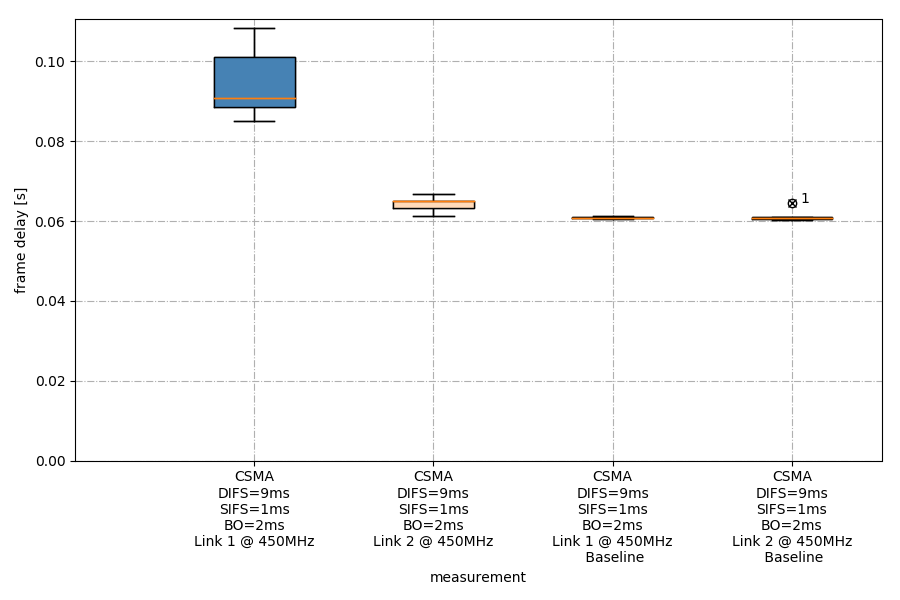
\includegraphics[width=0.6\textwidth]{pictures/results/same_combinations/csma_med_params/frame_delay_boxplot}}
		}
		\centerline{
			\subfloat[channel energy]{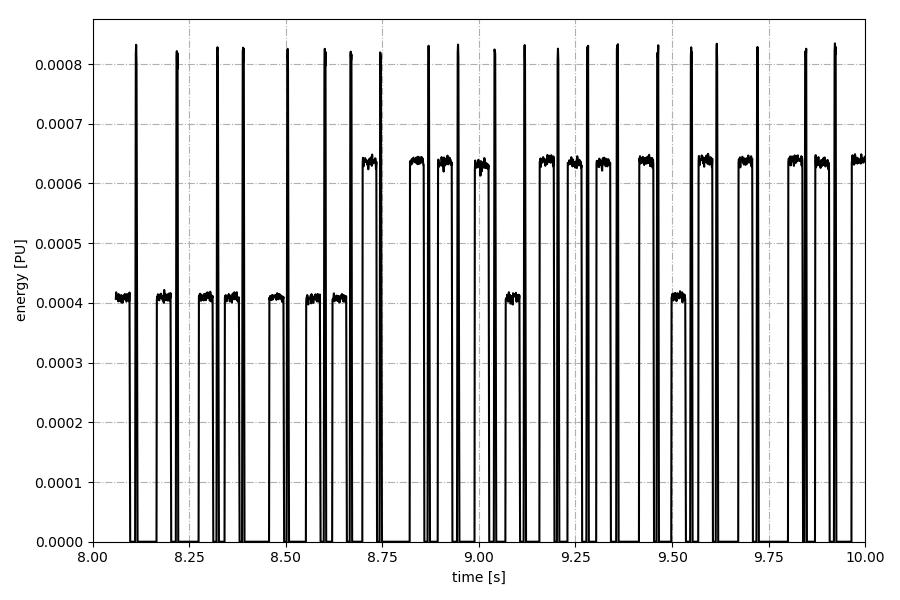
\includegraphics[width=0.6\textwidth]{pictures/results/same_combinations/csma_med_params/smoothed_channel_energy_level_4_line_chart}}
			\subfloat[channel energy CDF]{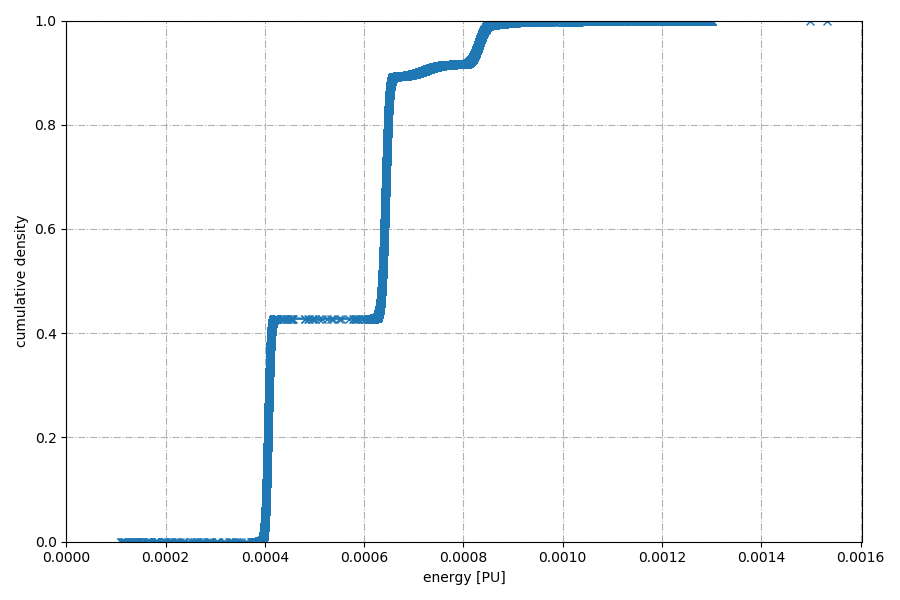
\includegraphics[width=0.6\textwidth]{pictures/results/same_combinations/csma_med_params/smoothed_channel_energy_cdf}}
		}
		\centerline{
			\subfloat[logical channel occupation]{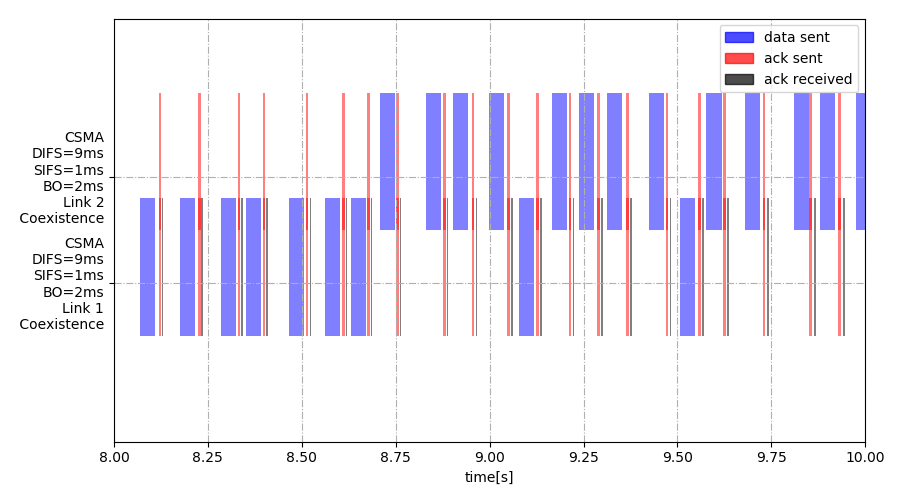
\includegraphics[width=0.6\textwidth]{pictures/results/same_combinations/csma_med_params/zoomed_channel_occupation_gantt_chart}}
			\subfloat[total backoff]{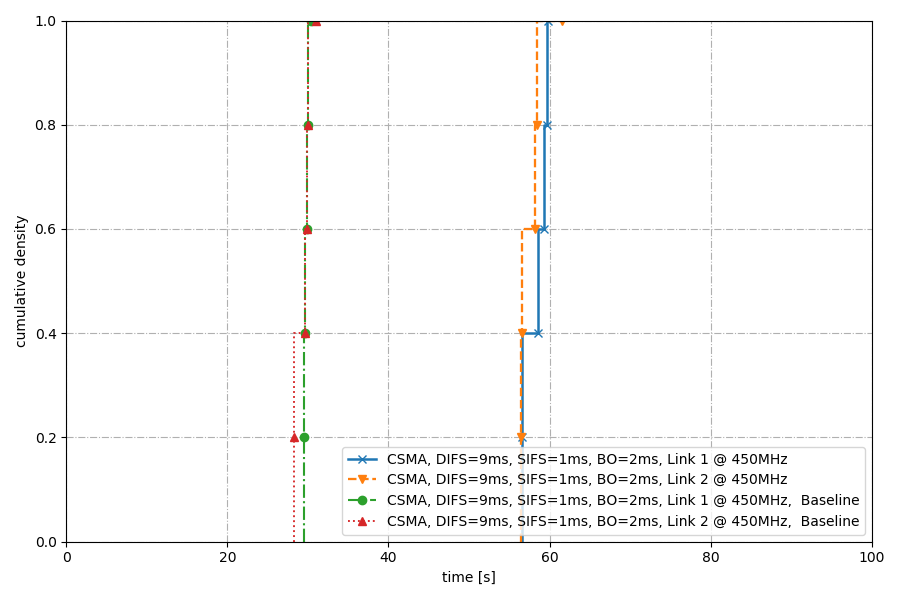
\includegraphics[width=0.6\textwidth]{pictures/results/same_combinations/csma_med_params/backoff_(joint)_sum_cdf}}
		}		
	\end{center}
	\caption{Measurement results for the CSMA/CA with medium parameter set}
\end{figure}

\clearpage



\subsection{1-persistent CSMA}

\begin{figure}[tb]
	\label{fig:results-difs-only-dbl}
	\begin{center}
		\centerline{
			\subfloat[throughput]{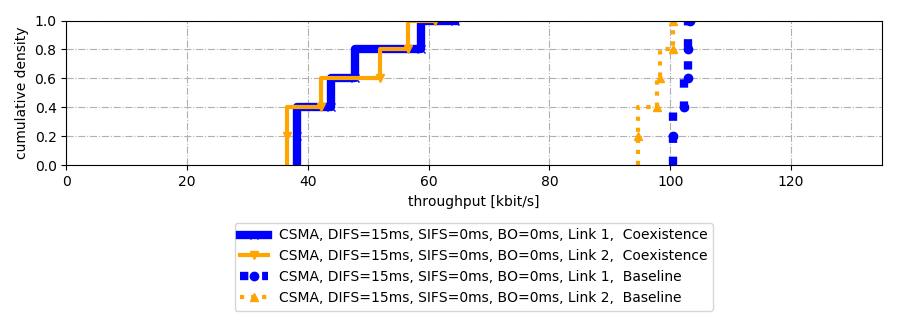
\includegraphics[width=0.6\textwidth]{pictures/results/same_combinations/difs_only/throughput_cdf}}
			\subfloat[frame delay]{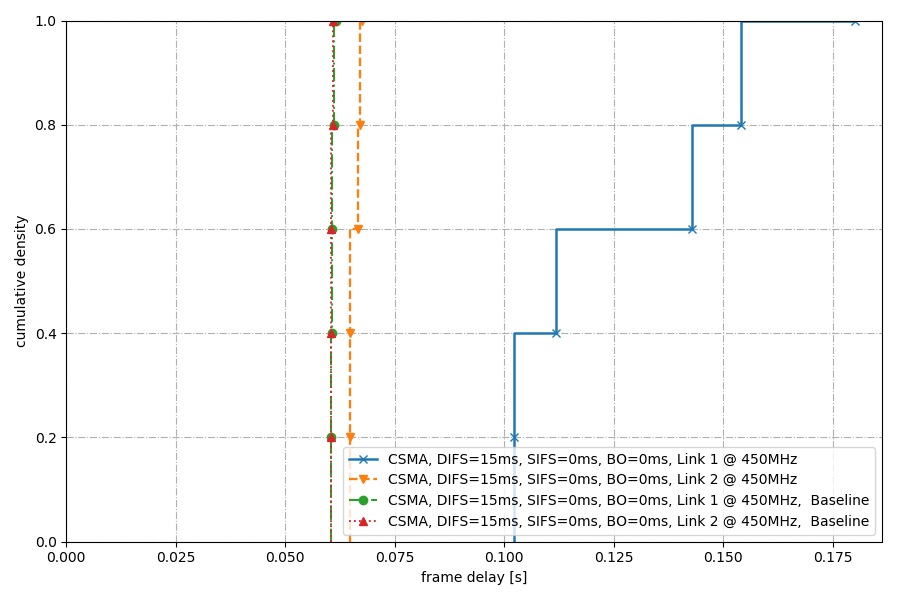
\includegraphics[width=0.6\textwidth]{pictures/results/same_combinations/difs_only/frame_delay_cdf}}
		}
		\centerline{
			\subfloat[Channel Energy]{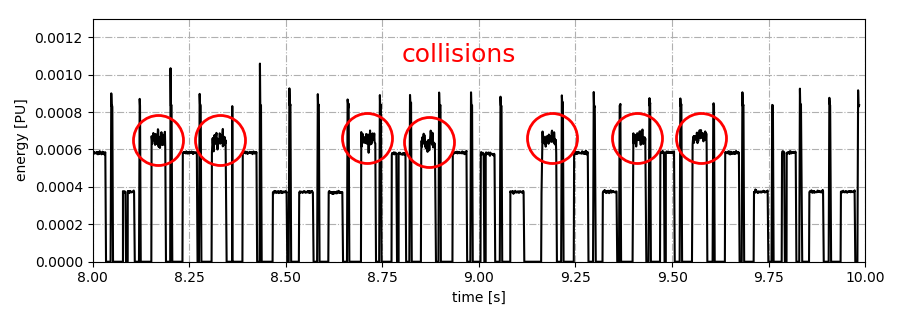
\includegraphics[width=0.6\textwidth]{pictures/results/same_combinations/difs_only/smoothed_channel_energy_level_4_line_chart}}
			\subfloat[Channel Energy CDF]{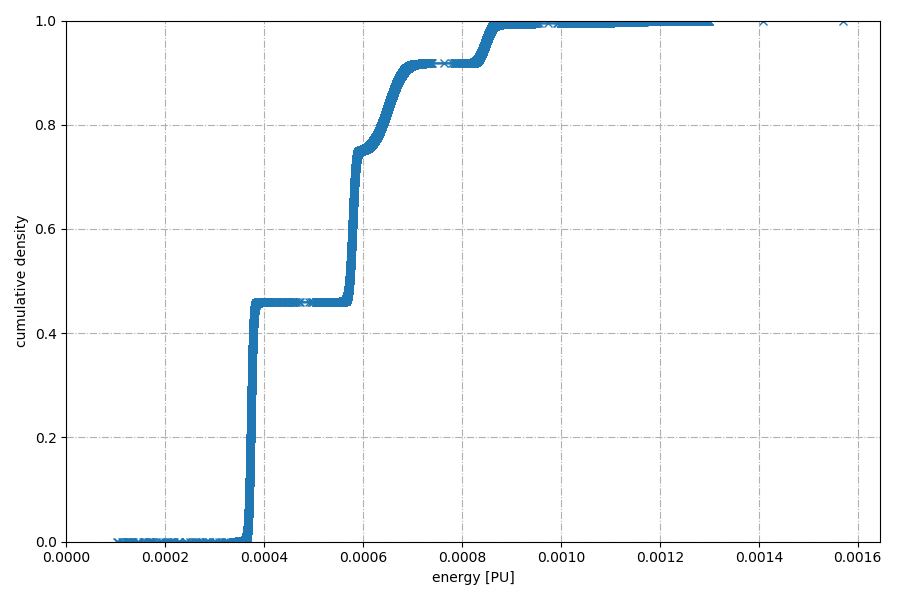
\includegraphics[width=0.6\textwidth]{pictures/results/same_combinations/difs_only/smoothed_channel_energy_cdf}}
		}
		\centerline{
			\subfloat[Logical Channel Occupation]{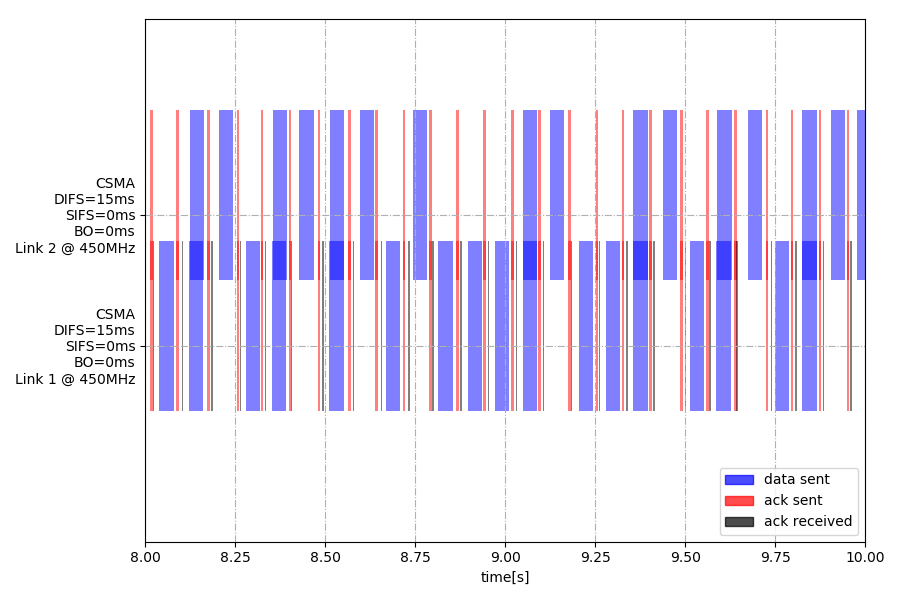
\includegraphics[width=0.6\textwidth]{pictures/results/same_combinations/difs_only/zoomed_channel_occupation_gantt_chart}}
			\subfloat[Total Backoff]{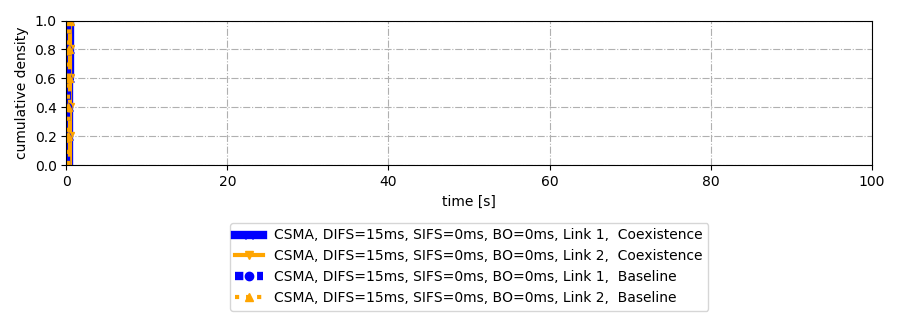
\includegraphics[width=0.6\textwidth]{pictures/results/same_combinations/difs_only/backoff_(joint)_sum_cdf}}
		}		
	\end{center}
	\caption{Measurement results for 1-persistent CSMA/CA}
\end{figure}

\clearpage




\section{Different Protocol Combinations}

%flawed
\subsection{ALOHA and CSMA/CA}

\begin{figure}[tb]
	\label{fig:results-aloha-csma}
	\begin{center}
		\centerline{
			\subfloat[Throughput]{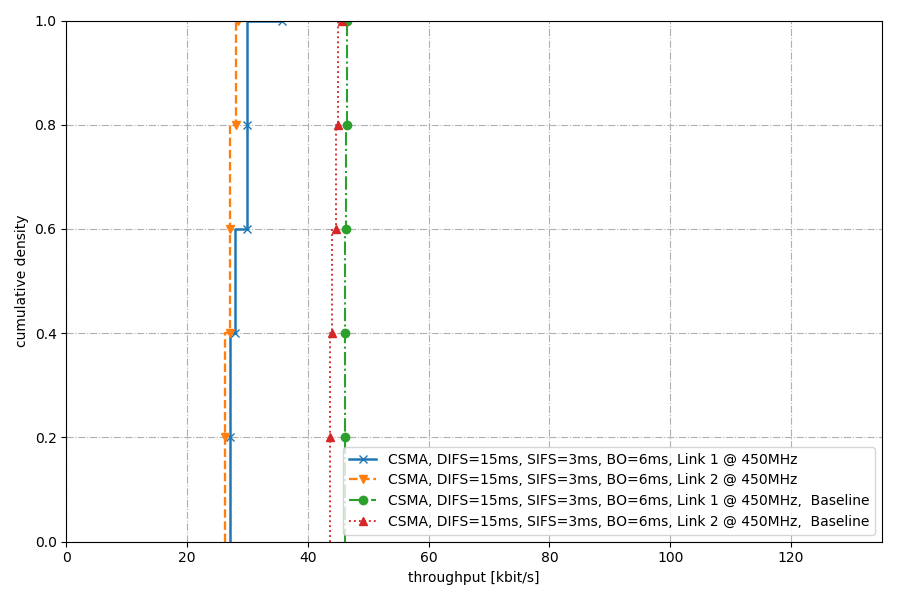
\includegraphics[width=0.6\textwidth]{pictures/results/same_combinations/csma_high_params/throughput_cdf}}
			\subfloat[RTT]{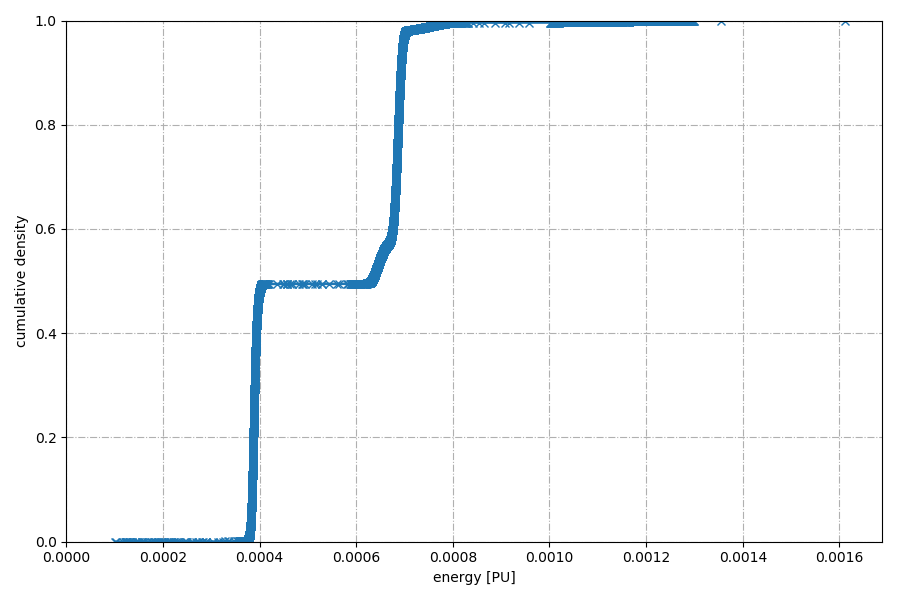
\includegraphics[width=0.6\textwidth]{pictures/results/same_combinations/csma_high_params/smoothed_channel_energy_cdf}}
		}
		\centerline{
			\subfloat[Channel Energy]{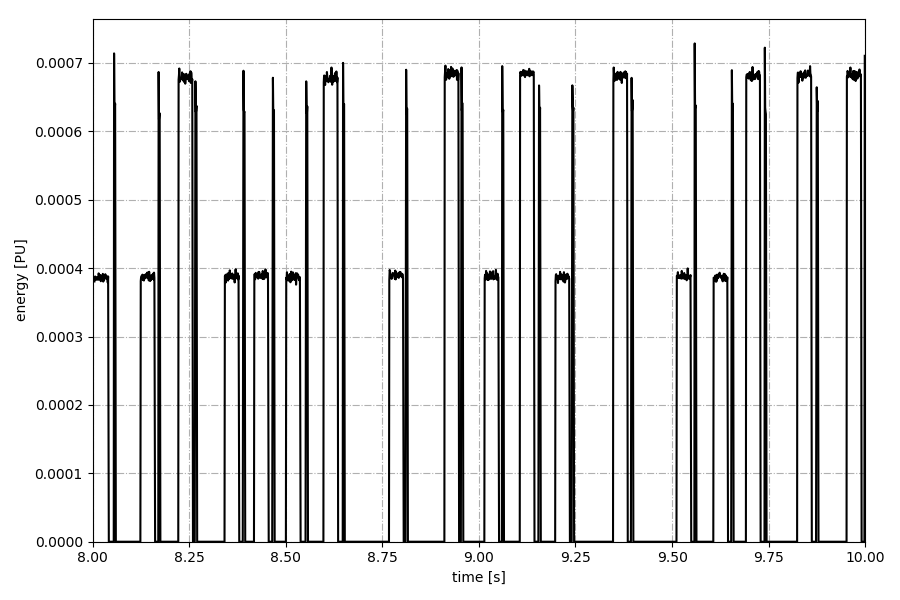
\includegraphics[width=0.6\textwidth]{pictures/results/same_combinations/csma_high_params/smoothed_channel_energy_level_4_line_chart}}
			\subfloat[Channel Energy CDF]{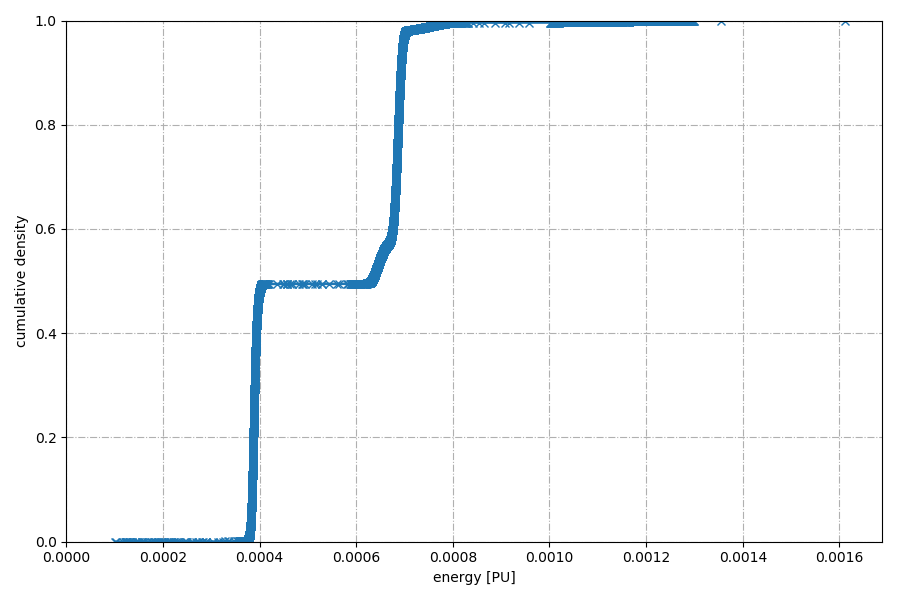
\includegraphics[width=0.6\textwidth]{pictures/results/same_combinations/csma_high_params/smoothed_channel_energy_cdf}}
		}
		\centerline{
			\subfloat[Logical Channel Occupation]{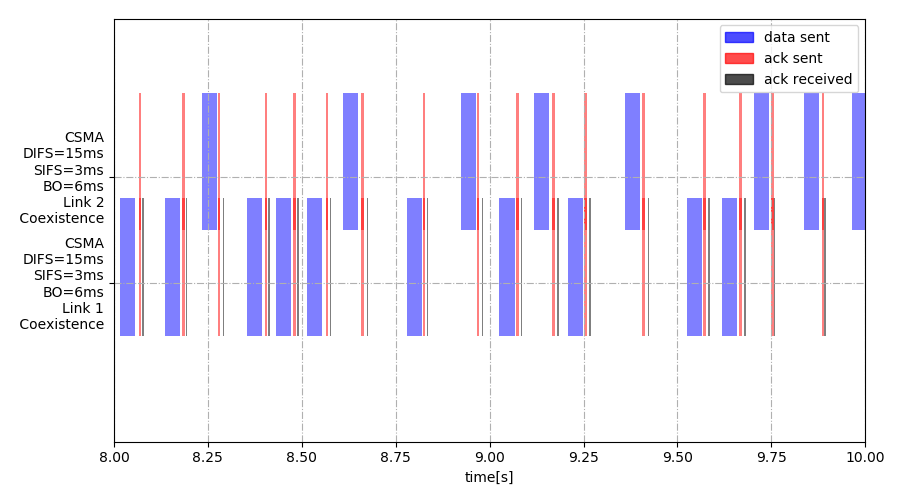
\includegraphics[width=0.6\textwidth]{pictures/results/same_combinations/csma_high_params/zoomed_channel_occupation_gantt_chart}}
			\subfloat[Total Backoff]{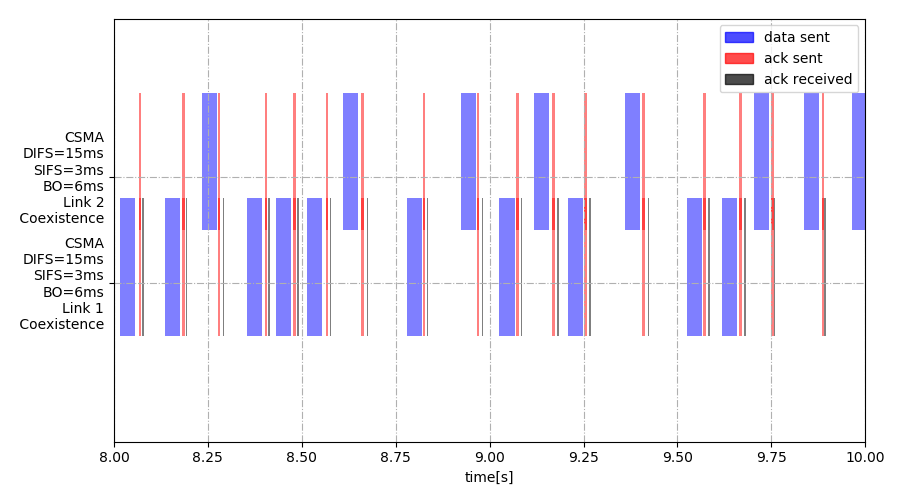
\includegraphics[width=0.6\textwidth]{pictures/results/same_combinations/csma_high_params/zoomed_channel_occupation_gantt_chart}}
		}		
	\end{center}
	\caption{Measurement results for the CSMA/CA with large parameter set}
\end{figure}

\clearpage



\subsection{Unsaturated ALOHA and CSMA/CA}

\begin{figure}[tb]
	\label{fig:results-unsat-aloha-csma}
	\begin{center}
		\centerline{
			\subfloat[Throughput]{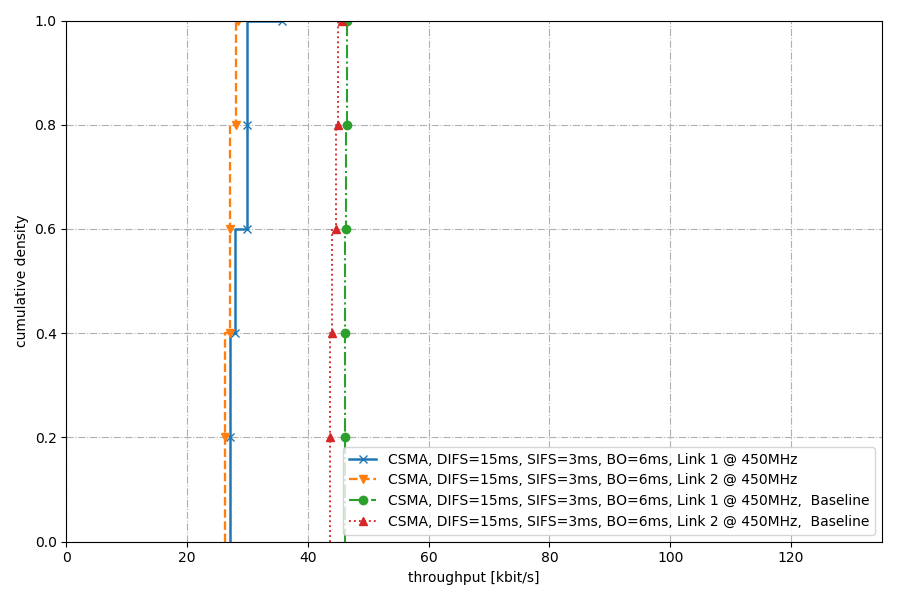
\includegraphics[width=0.6\textwidth]{pictures/results/same_combinations/csma_high_params/throughput_cdf}}
			\subfloat[RTT]{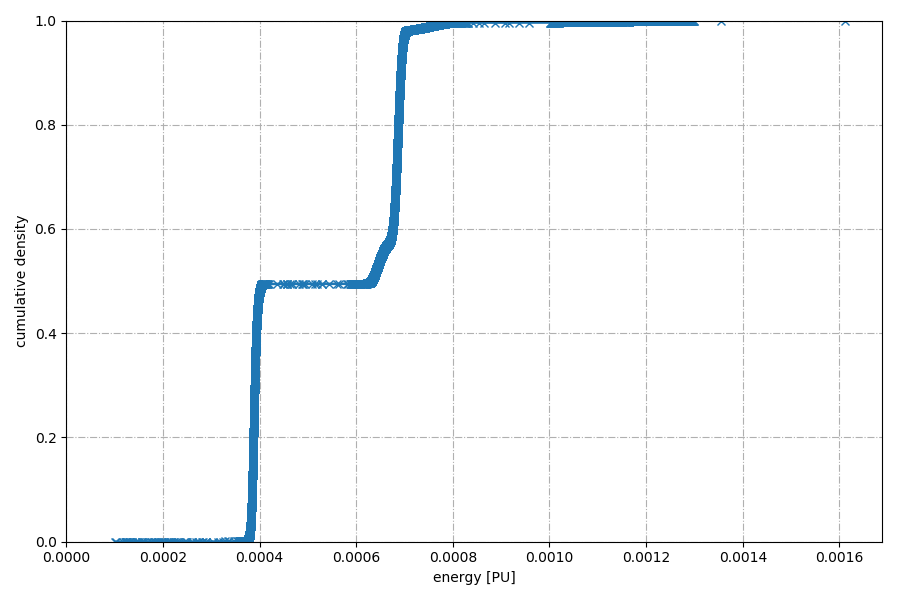
\includegraphics[width=0.6\textwidth]{pictures/results/same_combinations/csma_high_params/smoothed_channel_energy_cdf}}
		}
		\centerline{
			\subfloat[Channel Energy]{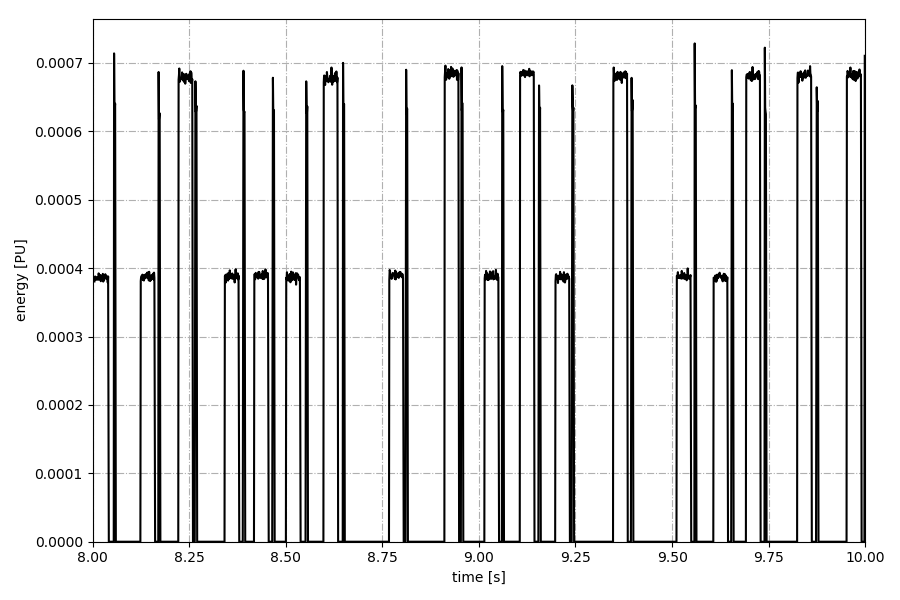
\includegraphics[width=0.6\textwidth]{pictures/results/same_combinations/csma_high_params/smoothed_channel_energy_level_4_line_chart}}
			\subfloat[Channel Energy CDF]{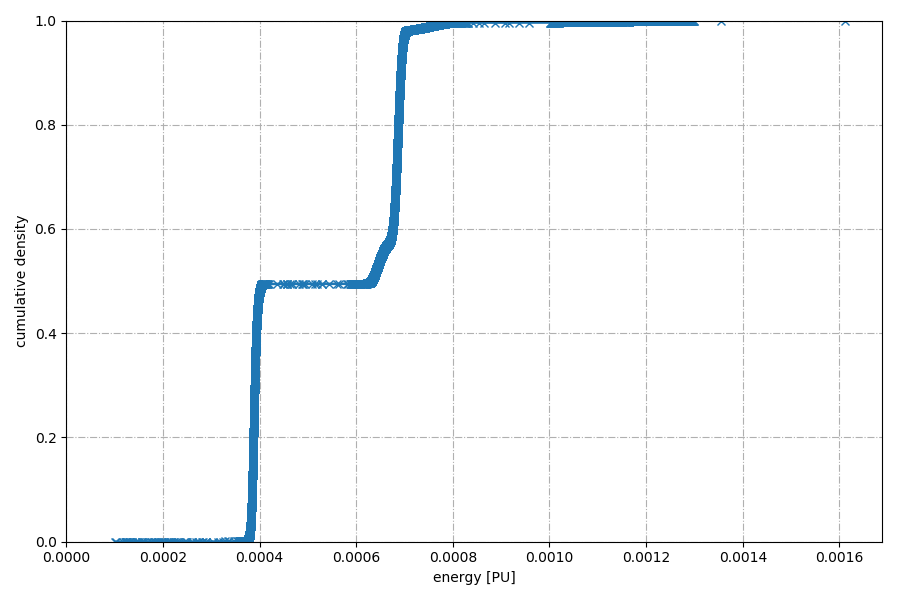
\includegraphics[width=0.6\textwidth]{pictures/results/same_combinations/csma_high_params/smoothed_channel_energy_cdf}}
		}
		\centerline{
			\subfloat[Logical Channel Occupation]{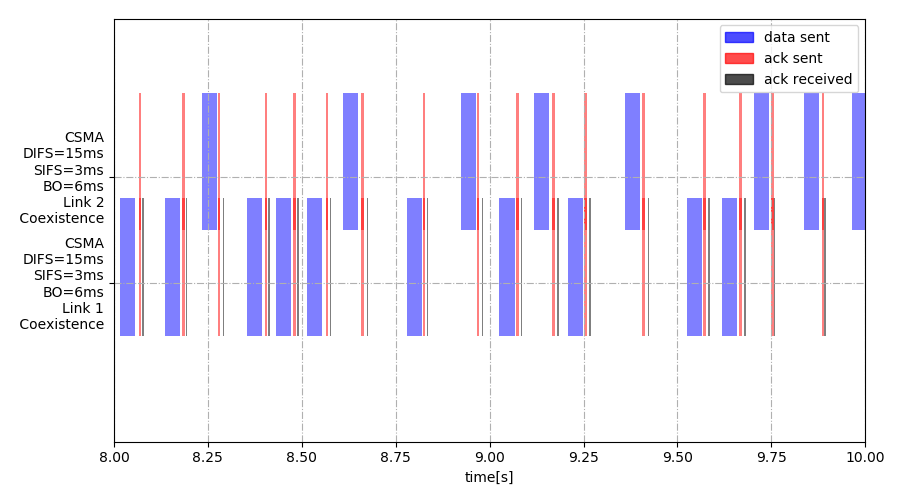
\includegraphics[width=0.6\textwidth]{pictures/results/same_combinations/csma_high_params/zoomed_channel_occupation_gantt_chart}}
			\subfloat[Total Backoff]{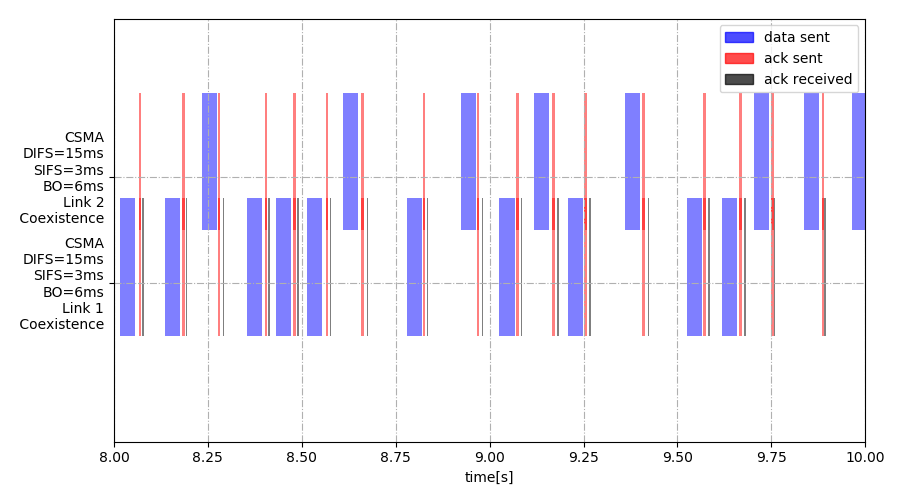
\includegraphics[width=0.6\textwidth]{pictures/results/same_combinations/csma_high_params/zoomed_channel_occupation_gantt_chart}}
		}		
	\end{center}
	\caption{Measurement results for the CSMA/CA with large parameter set}
\end{figure}

\clearpage




\subsection{Inhomogeneous CSMA/CA }



\subsection{1-persistent CSMA and ALOHA}

\begin{figure}[tb]
	\label{fig:results-difs-aloha}
	\begin{center}
		\centerline{
			\subfloat[Throughput]{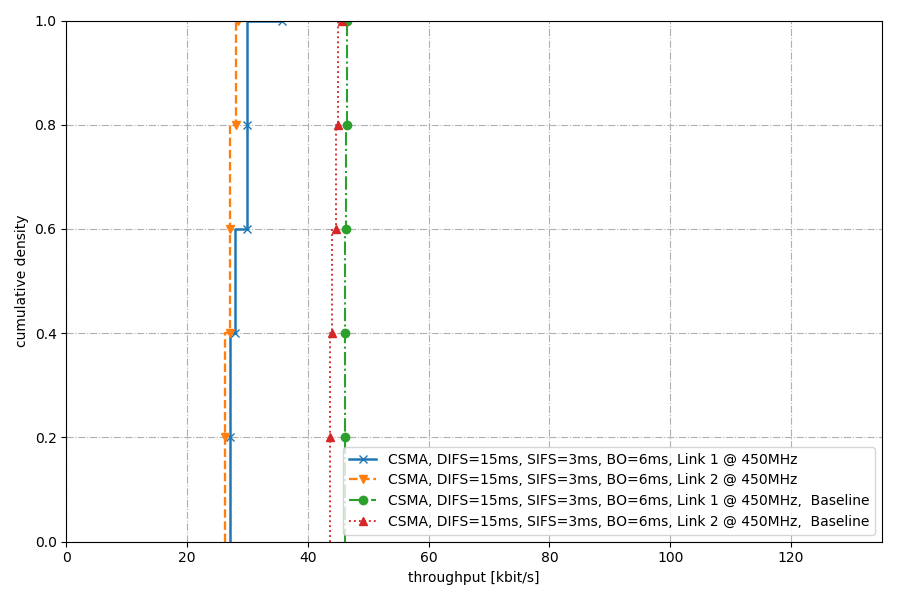
\includegraphics[width=0.6\textwidth]{pictures/results/same_combinations/csma_high_params/throughput_cdf}}
			\subfloat[RTT]{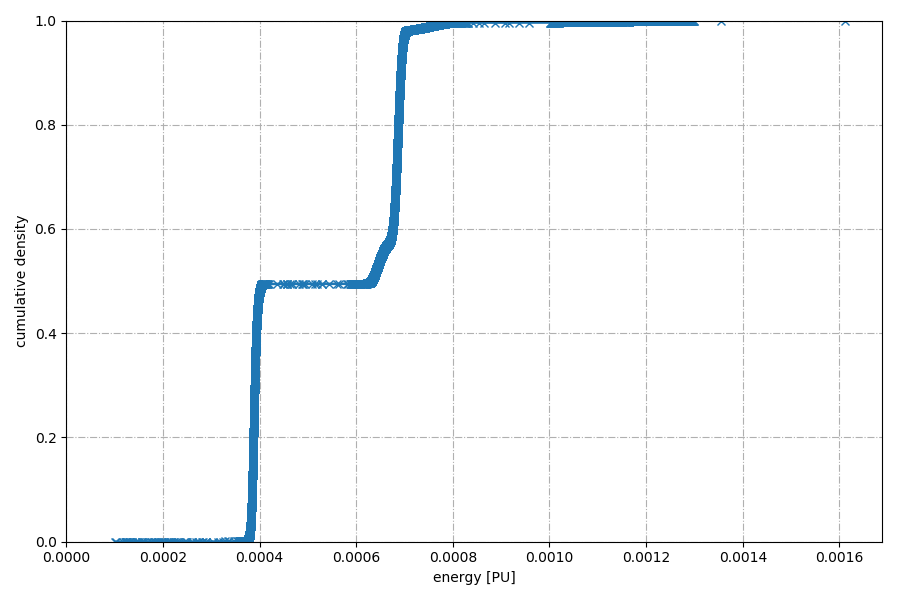
\includegraphics[width=0.6\textwidth]{pictures/results/same_combinations/csma_high_params/smoothed_channel_energy_cdf}}
		}
		\centerline{
			\subfloat[Channel Energy]{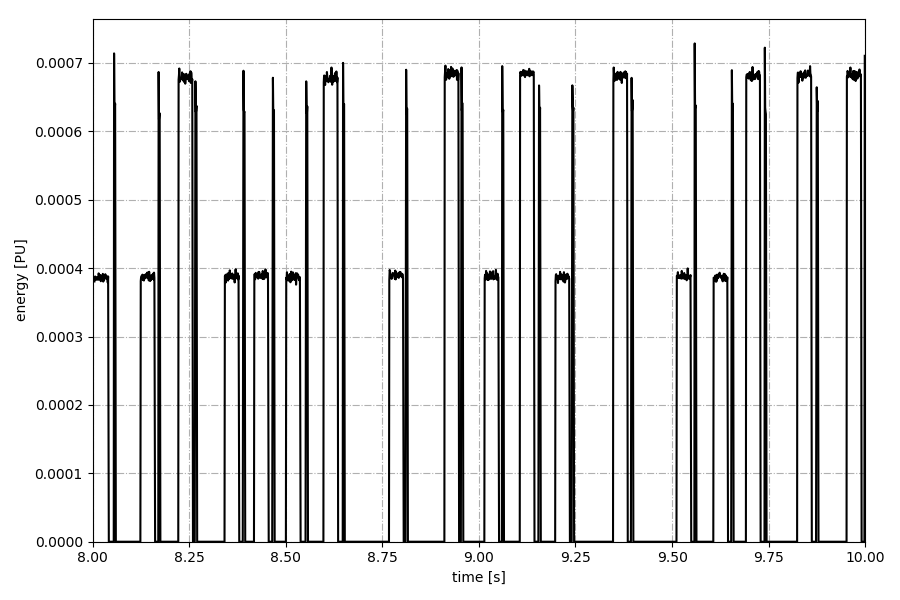
\includegraphics[width=0.6\textwidth]{pictures/results/same_combinations/csma_high_params/smoothed_channel_energy_level_4_line_chart}}
			\subfloat[Channel Energy CDF]{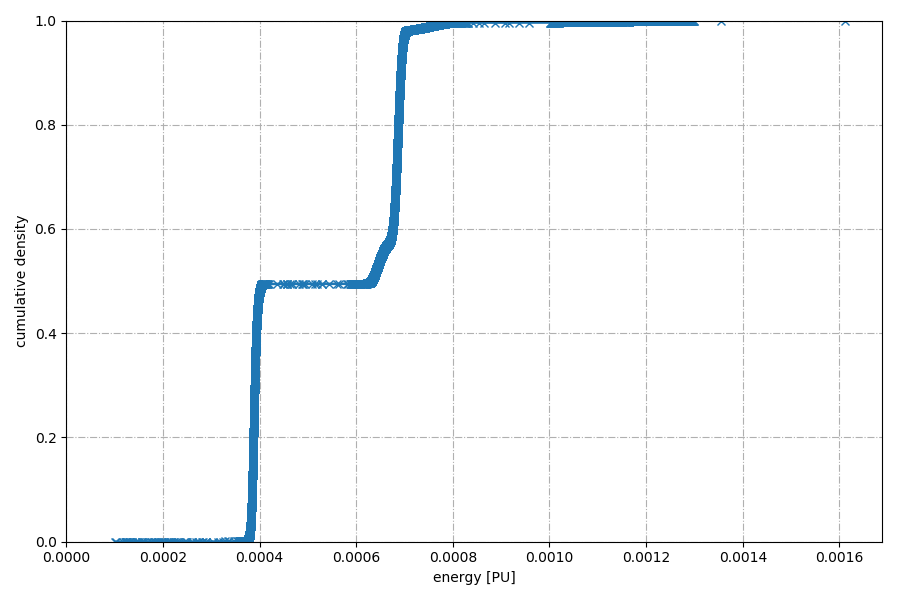
\includegraphics[width=0.6\textwidth]{pictures/results/same_combinations/csma_high_params/smoothed_channel_energy_cdf}}
		}
		\centerline{
			\subfloat[Logical Channel Occupation]{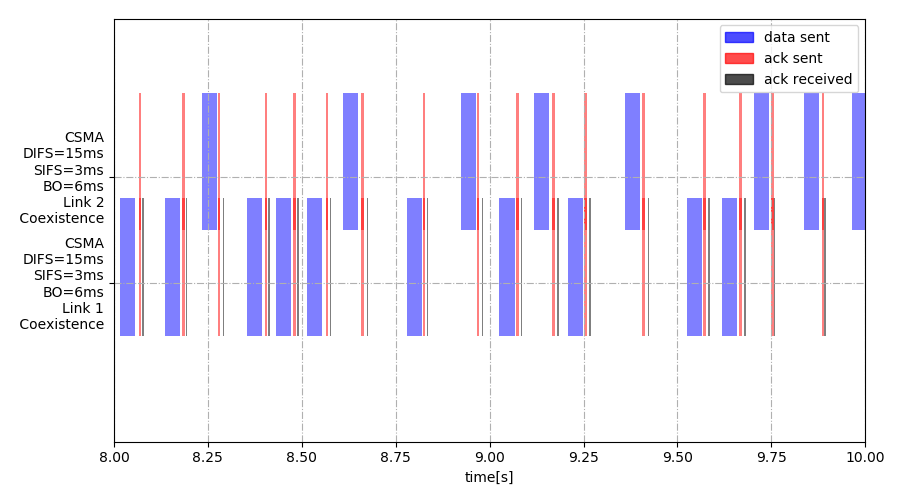
\includegraphics[width=0.6\textwidth]{pictures/results/same_combinations/csma_high_params/zoomed_channel_occupation_gantt_chart}}
			\subfloat[Total Backoff]{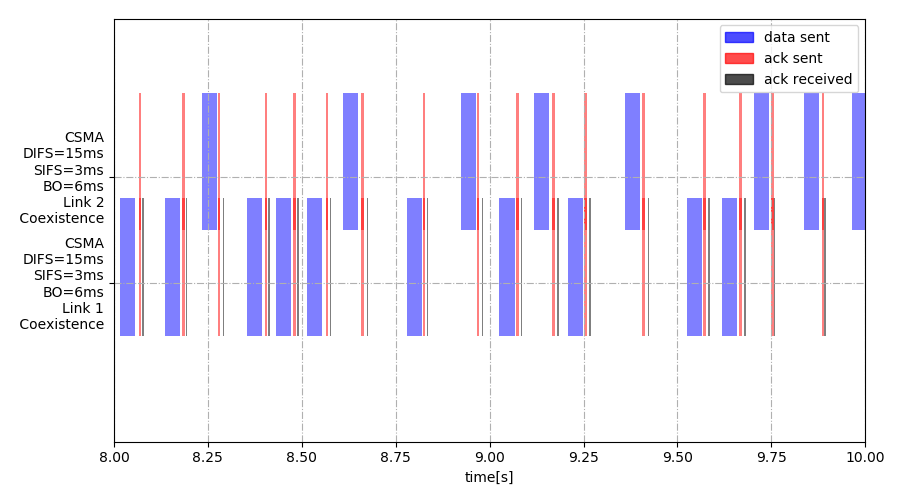
\includegraphics[width=0.6\textwidth]{pictures/results/same_combinations/csma_high_params/zoomed_channel_occupation_gantt_chart}}
		}		
	\end{center}
	\caption{Measurement results for the CSMA/CA with large parameter set}
\end{figure}

\clearpage



\subsection{1-persistent CSMA and CSMA/CA}

\begin{figure}[tb]
	\label{fig:results-difs-csma}
	\begin{center}
		\centerline{
			\subfloat[Throughput]{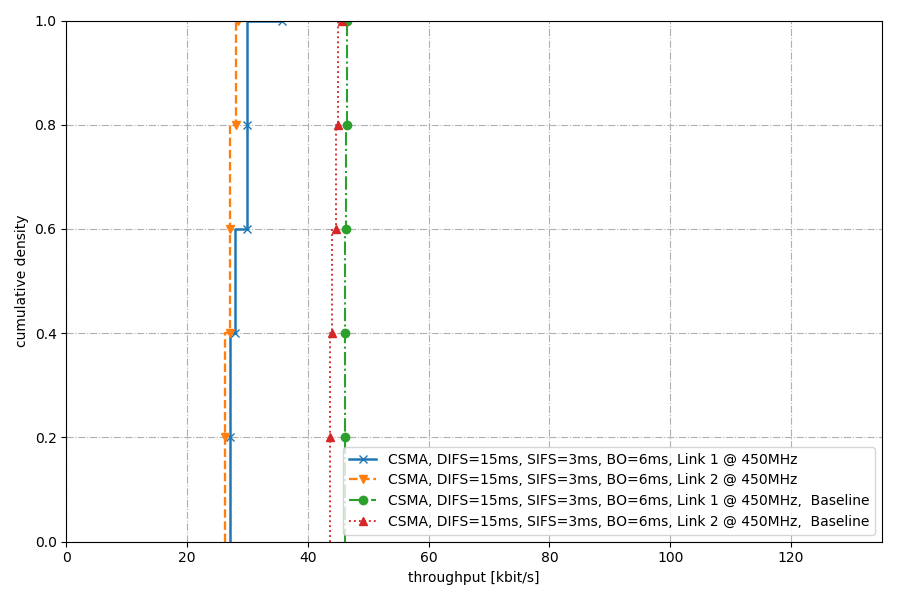
\includegraphics[width=0.6\textwidth]{pictures/results/same_combinations/csma_high_params/throughput_cdf}}
			\subfloat[RTT]{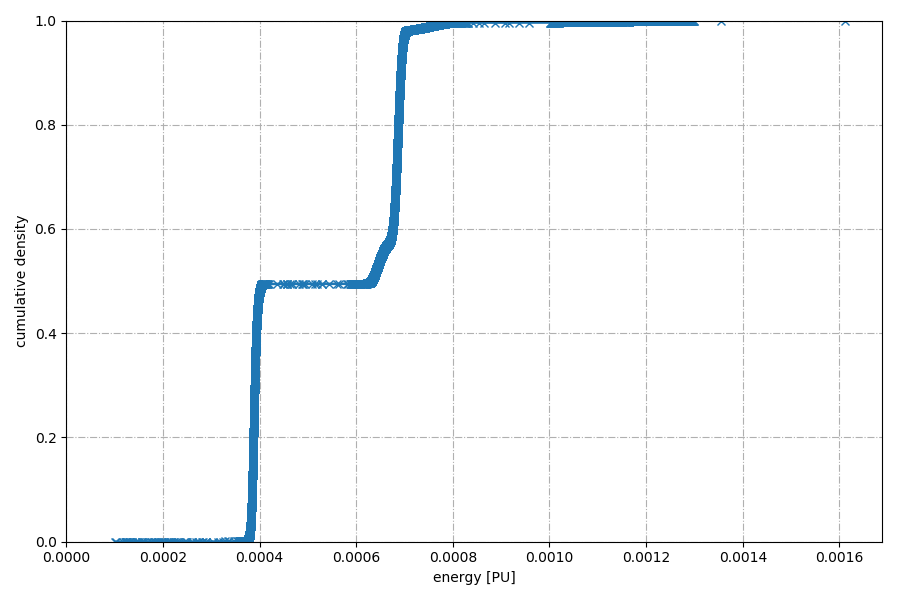
\includegraphics[width=0.6\textwidth]{pictures/results/same_combinations/csma_high_params/smoothed_channel_energy_cdf}}
		}
		\centerline{
			\subfloat[Channel Energy]{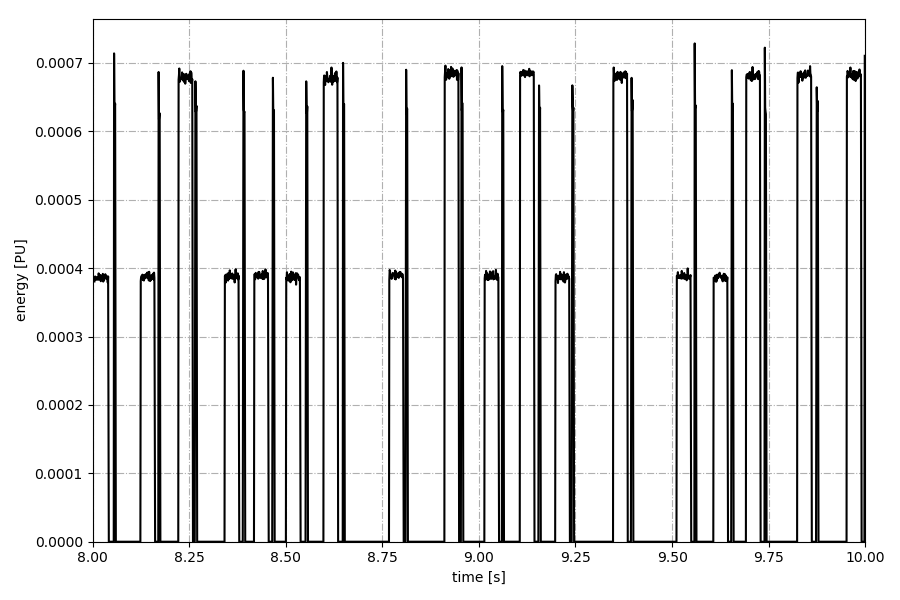
\includegraphics[width=0.6\textwidth]{pictures/results/same_combinations/csma_high_params/smoothed_channel_energy_level_4_line_chart}}
			\subfloat[Channel Energy CDF]{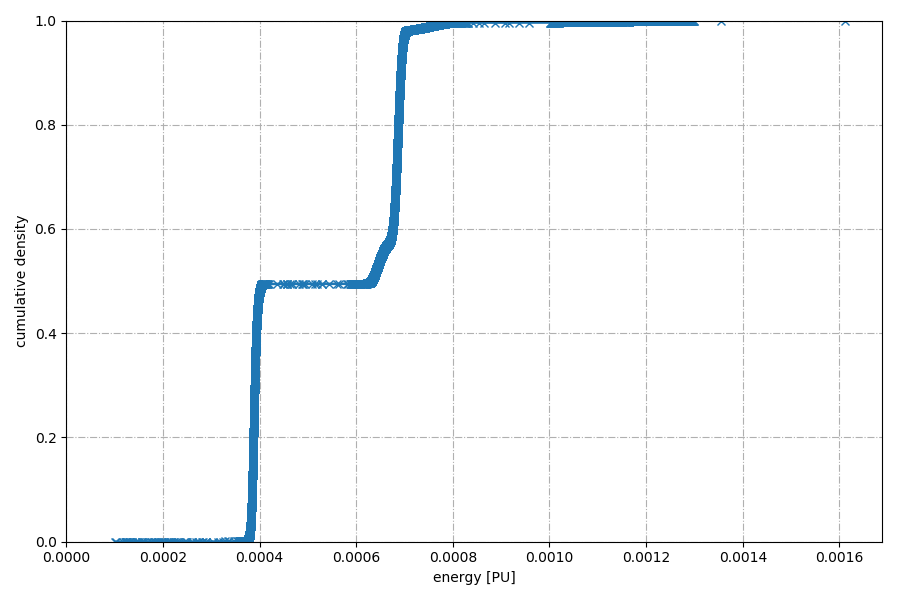
\includegraphics[width=0.6\textwidth]{pictures/results/same_combinations/csma_high_params/smoothed_channel_energy_cdf}}
		}
		\centerline{
			\subfloat[Logical Channel Occupation]{\includegraphics[width=0.6\textwidth]{pictures/results/same_combinations/csma_high_params/zoomed_channel_occupation_gantt_chart}}
			\subfloat[Total Backoff]{\includegraphics[width=0.6\textwidth]{pictures/results/same_combinations/csma_high_params/zoomed_channel_occupation_gantt_chart}}
		}		
	\end{center}
	\caption{Measurement results for the CSMA/CA with large parameter set}
\end{figure}